\chapter{Diseño de la interfaz de usuario}

Una vez hemos definido cuáles son nuestros objetivos, analizado el estado del arte y establecido unas pautas para el desarrollo, vamos a comenzar con el diseño de la parte visual. Esto es, a su vez, un proceso que requiere de distintas definiciones, de manera que al término de este capítulo, no sólo tengamos el diseño de las interfaces de usuario, sino que también comprendamos por qué se han diseñado así y la intención de cada elemento que disponemos en pantalla.

\section{Matriz de tareas de usuario}

Un buen comienzo sería el de definir los roles de usuario en nuestra nueva aplicación. Hemos hablado ya en el capítulo anterior sobre la figura del \gls{gestortwinX} y la del \gls{superusuario}. Incluyamos entonces también las de \gls{Tutor}, estudiante y, de forma excepcional, la de coordinador(a) externo/a. Sobre esta última, recordemos que no tenía ningún tipo de interacción en TWINS y que hasta entonces, los usuarios de la plataforma habían establecido intercambios de información por correo electrónico con los coordinadores de otras facultades, que es el método estándar de realizar las \glspl{Nominacion}. Sin embargo, aunque no para sus primeras versiones, se espera que twinX brinde la capacidad de hacer estas nominaciones a través de una interfaz gráfica, de una forma mucho más sencilla y segura que con el envío de un texto libre, donde puede haber errores y/o malas prácticas, dado el amplio uso que se puede hacer de la herramienta.

Es precisamente por la necesidad de dejar claras las acciones a llevar a cabo por cada usuario del sistema por la que elaborar una \textbf{matriz de tareas de usuario}. Esta herramienta nos permite establecer cuál es la frecuencia de uso de una característica de nuestra aplicación por un grupo de usuarios en concreto y cuál es la prioridad que debemos darle a la implementación de la misma. De esta forma, nos será más fácil diferenciar aquellas acciones que tan solo se lleven a cabo unas pocas veces al mes (o cada varios meses) y cuales, por el contrario, son ejecutadas casi a diario, de modo que se priorice su integración y su optimización. Sobre estas últimas, cabe decir que el potenciarlas no solo se procurará hacer en términos de procesamiento interno del código, sino también en cuanto a su facilidad de utilización por parte del usuario. Es decir, tendremos que crear más accesos directos o simplificar lo máximo posible el curso de tareas a llevar a cabo para realizar estas acciones y obtener los resultados deseados. En adición a todo esto, podremos observar cuáles son los usuarios que menos usarán la plataforma, de modo que se reste prioridad a la implementación de sus interacciones, en beneficio de las que llevan a cabo los usuarios que, por el contrario, monopolizan el uso de la aplicación.

\section{Sitemap}
\section{Labelling (iconografía)}
\section{Bocetos wireframe}

\subsection{Wireframes del módulo de gestión}

\begin{figure}
	\centering
	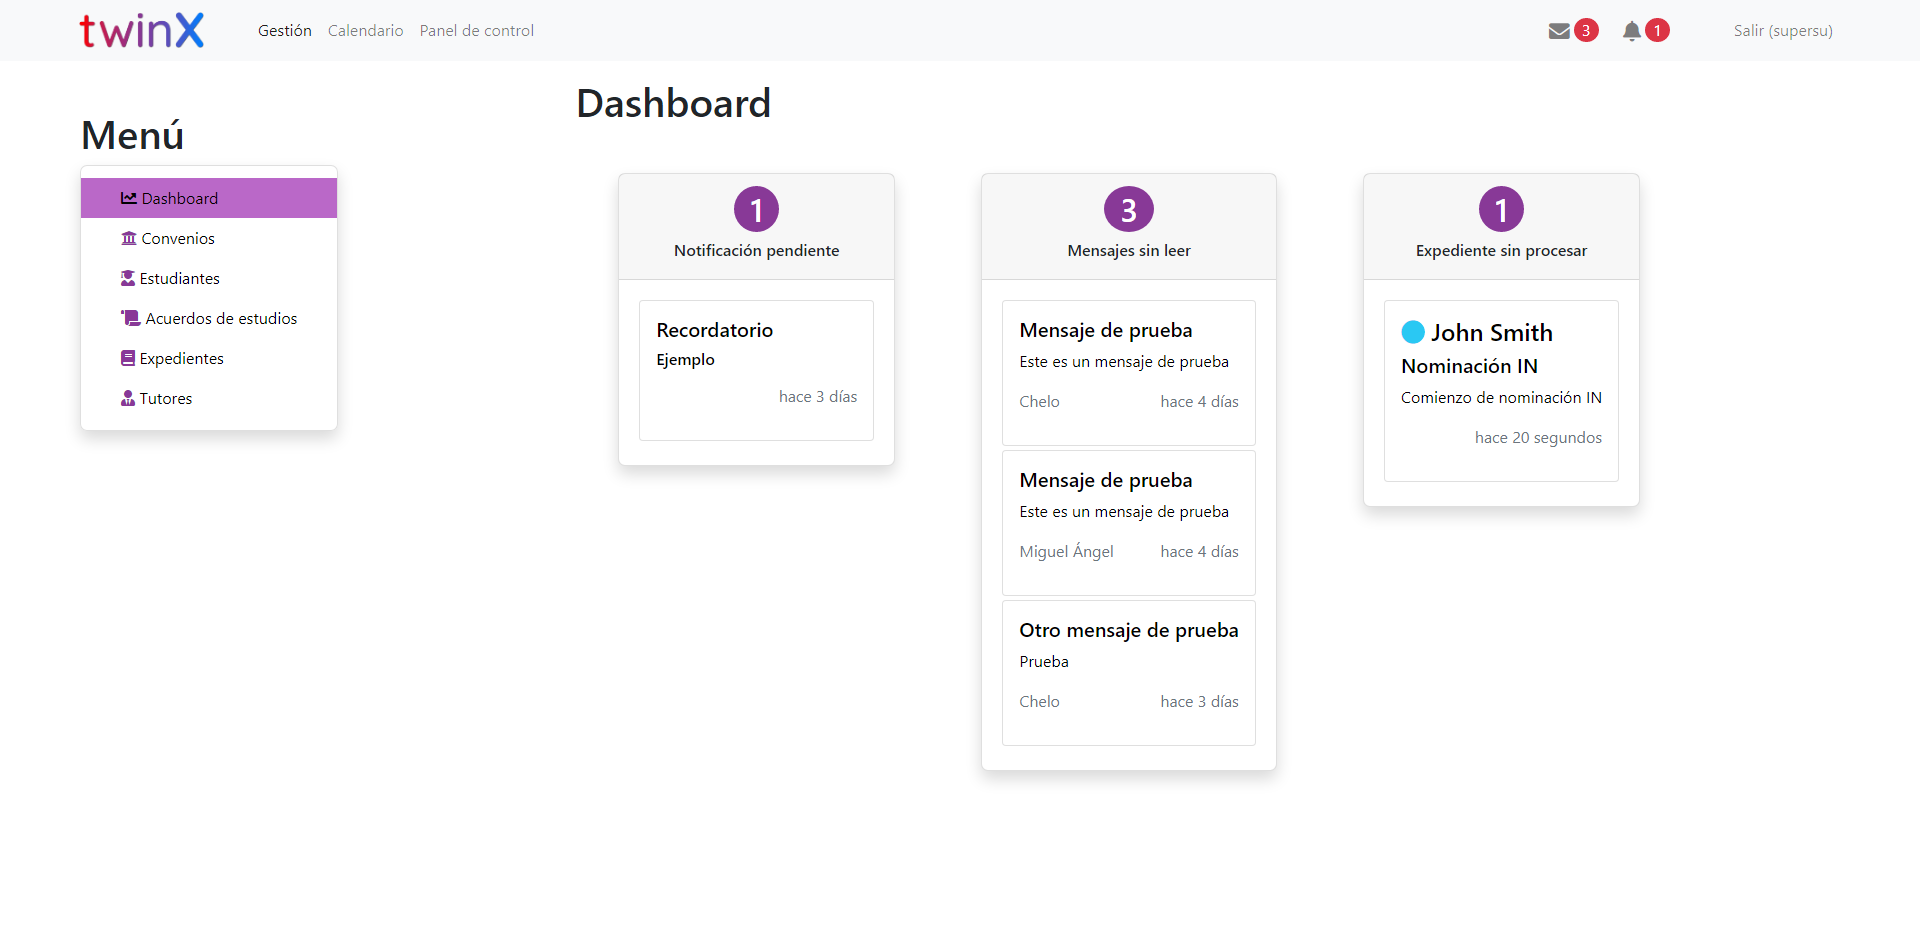
\includegraphics[width=\textwidth]{img/Wireframes/Gestión/dashboard.png}
	\caption[Wireframe de \textit{Dashboard}]{Wireframe del \textit{Dashboard} donde el usuario verá de un vistazo toda la información de mayor importancia al iniciar la aplicación}
	\label{fig:dashboardWF}
\end{figure}

\begin{figure}
	\centering
	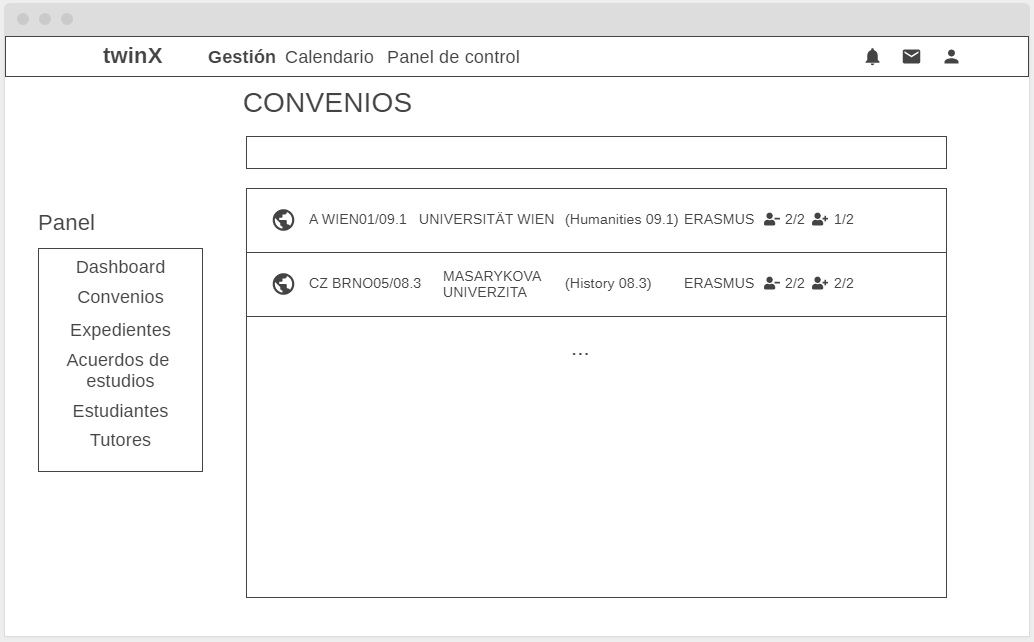
\includegraphics[width=\textwidth]{img/Wireframes/Gestión/convenios_lista.png}
	\caption{Wireframe de lista de convenios}
	\label{fig:convenios_listaWF}
\end{figure}

\begin{figure}
\centering
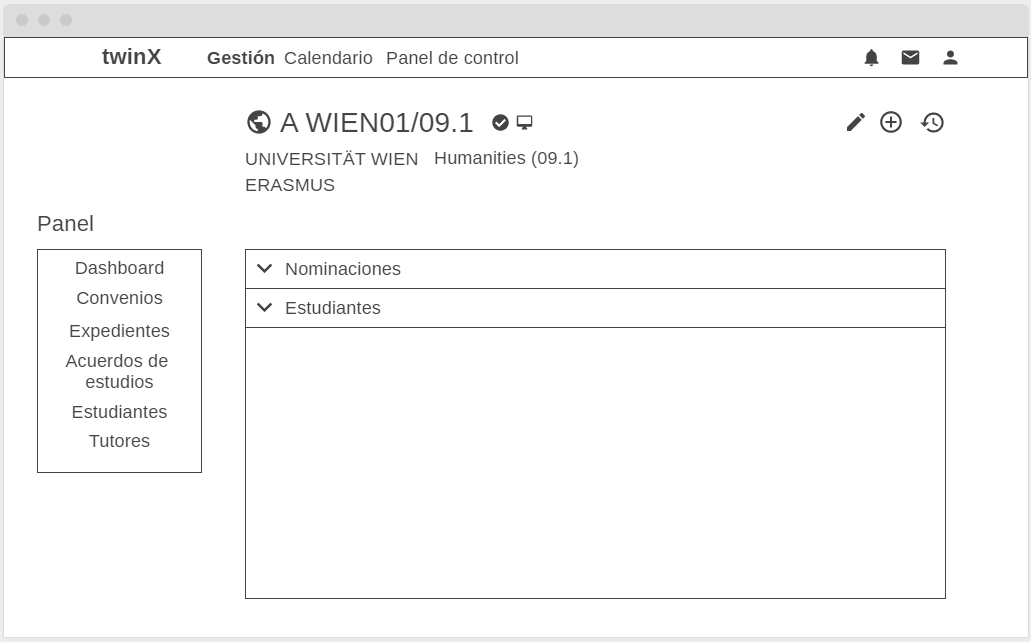
\includegraphics[width=\textwidth]{img/Wireframes/Gestión/vista_convenio_básica_contraída.png}
\caption[Wireframe de vista de convenio básica]{Wireframe de vista de convenio básica. Secciones contraídas.}
\label{fig:vista_conv_básica_contWF}
\end{figure}

\begin{figure}
	\centering
	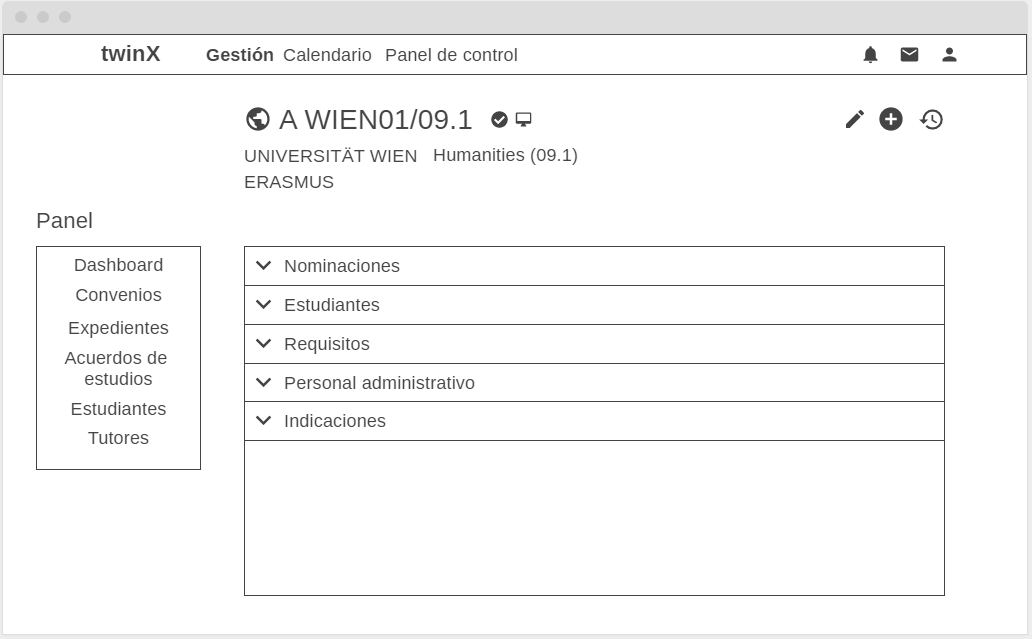
\includegraphics[width=\textwidth]{img/Wireframes/Gestión/vista_convenio_avanzada_contraída.png}
	\caption[Wireframe de vista de convenio avanzada]{Wireframe de vista de convenio avanzada. Secciones contraídas. Acceso desde el botón «+» de la botonera en la esquina superior derecha del contenido principal.}
	\label{fig:vista_conv_avanzada_contWF}
\end{figure}

\begin{figure}
	\centering
	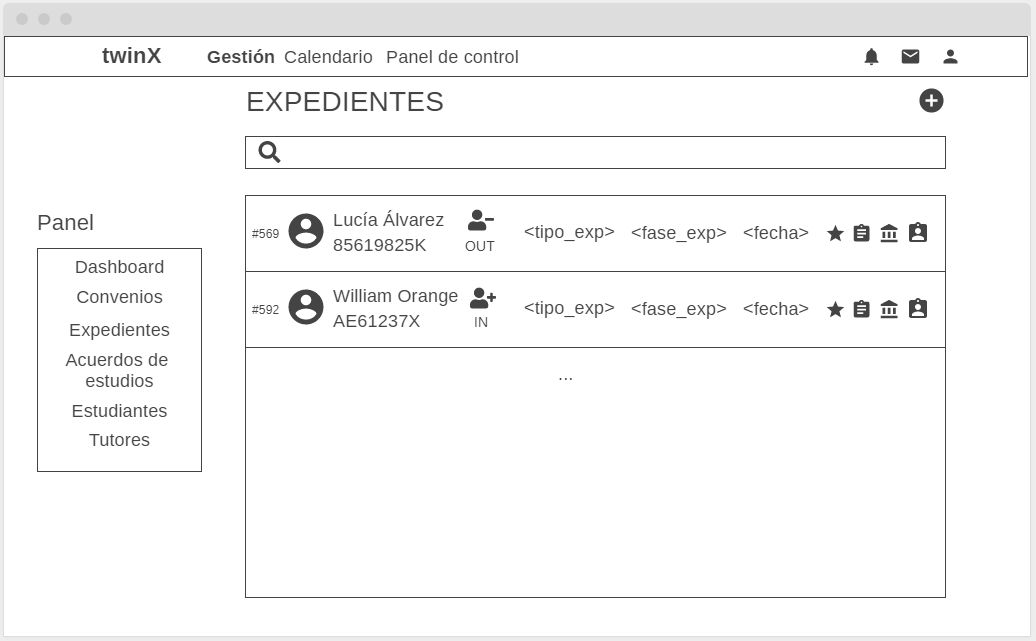
\includegraphics[width=\textwidth]{img/Wireframes/Gestión/expedientes_lista.png}
	\caption{Wireframe de lista de expedientes}
	\label{fig:expedientes_listaWF}
\end{figure}

\begin{figure}
	\centering
	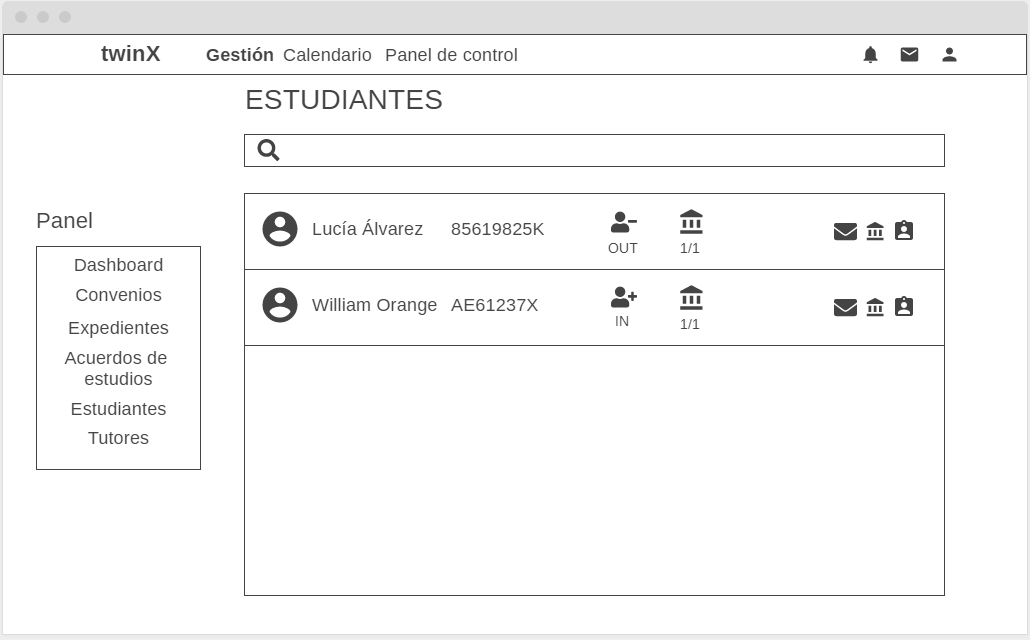
\includegraphics[width=\textwidth]{img/Wireframes/Gestión/estudiantes_lista.png}
	\caption{Wireframe de lista de estudiantes}
	\label{fig:estudiantes_listaWF}
\end{figure}

\begin{figure}
	\centering
	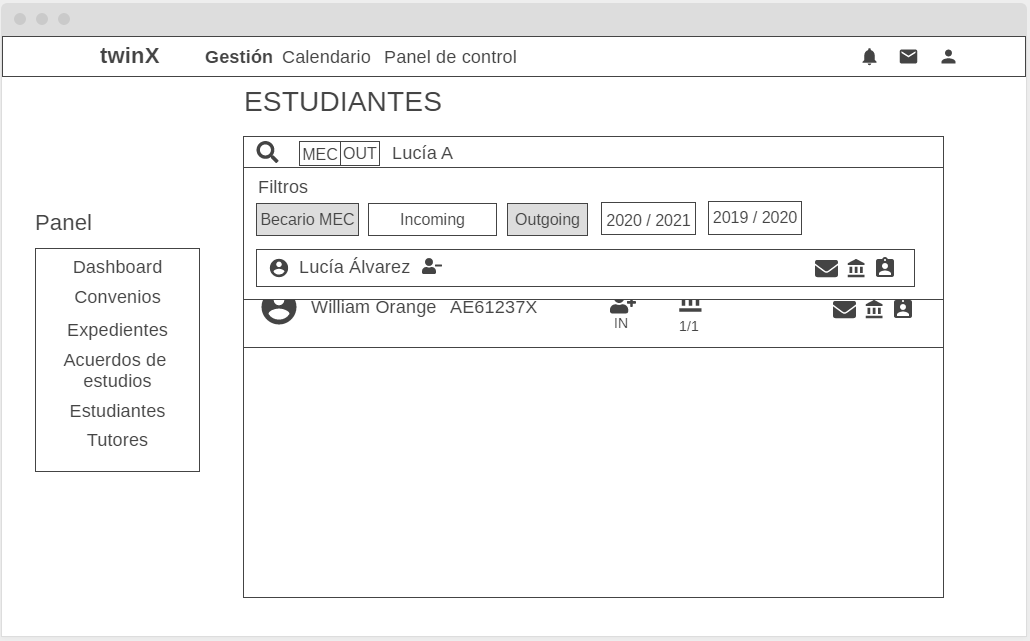
\includegraphics[width=\textwidth]{img/Wireframes/Gestión/búsqueda.png}
	\caption[Wireframe de búsqueda]{Wireframe de búsqueda. Diálogo modal, desplegable desde la barra. Capacidad de filtrado}
	\label{fig:búsquedaWF}
\end{figure}

\begin{figure}
	\centering
	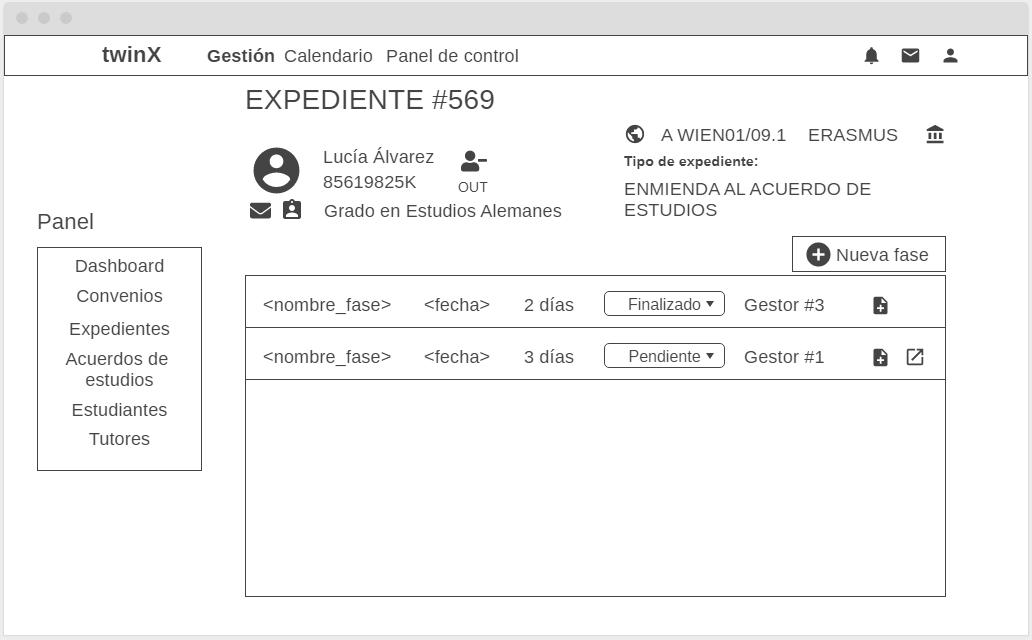
\includegraphics[width=\textwidth]{img/Wireframes/Gestión/expediente_detalle.png}
	\caption{Wireframe de detalle de expediente}
	\label{fig:expediente_detalleWF}
\end{figure}

\begin{figure}
	\centering
	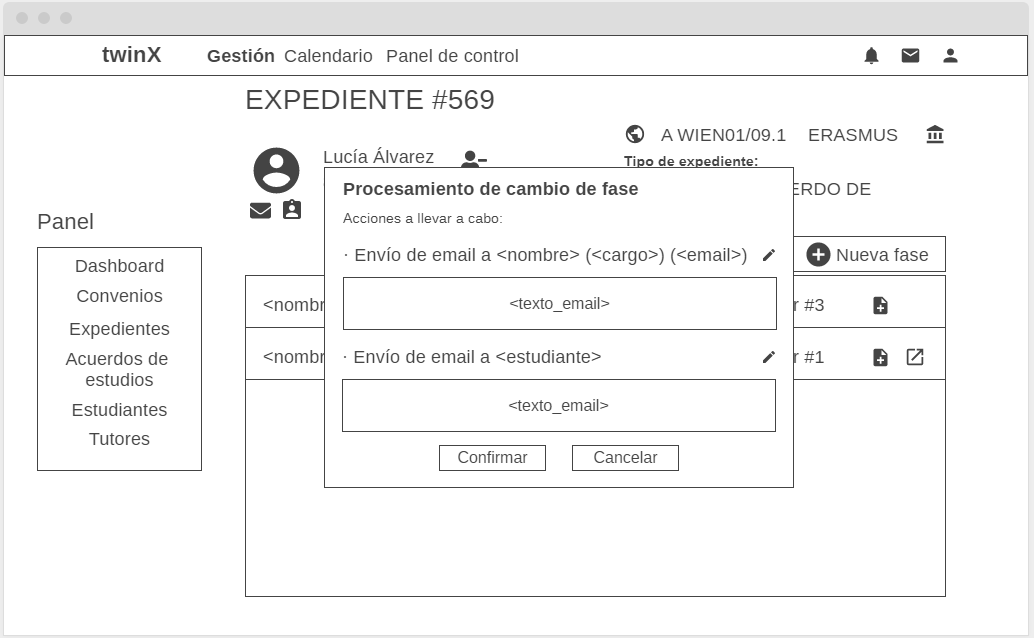
\includegraphics[width=\textwidth]{img/Wireframes/Gestión/cambio_fase.png}
	\caption[Wireframe del modal de cambio de fase]{Wireframe del modal de cambio de fase. Advierte sobre las acciones a llevar a cabo tras la tramitación del cambio de fase en un expediente concreto.}
	\label{fig:cambio_faseWF}
\end{figure}

\begin{figure}
	\centering
	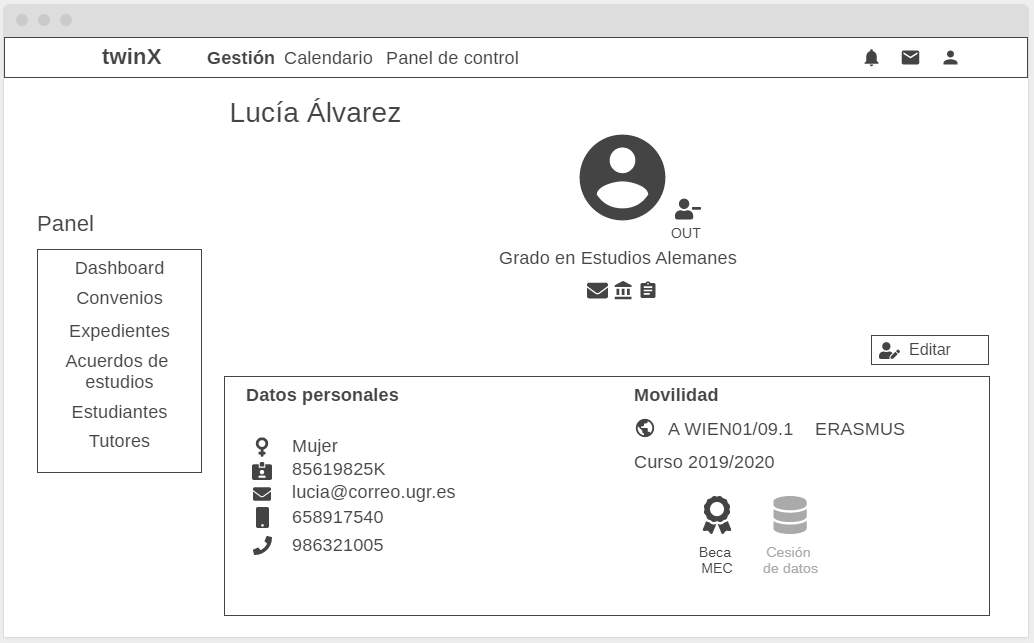
\includegraphics[width=\textwidth]{img/Wireframes/Gestión/estudiante_detalle.png}
	\caption{Wireframe de la vista de detalle de un estudiante}
	\label{fig:estudiante_detalleWF}
\end{figure}

%%PROVISIONAL PARA SEPARAR AMBOS CONJUNTOS DE WIREFRAMES
\newpage

\subsection{Wireframes del módulo de calendario}

\begin{figure}
	\centering
	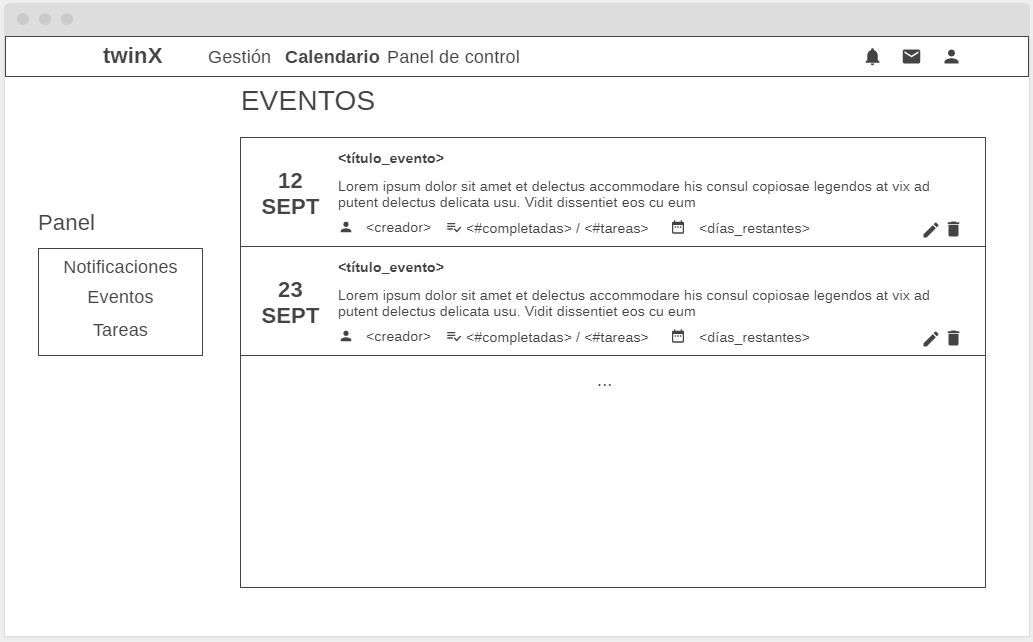
\includegraphics[width=\textwidth]{img/Wireframes/Calendario/eventos_lista.png}
	\caption{Wireframe de lista de eventos}
	\label{fig:eventos_listaWF}
\end{figure}

\begin{figure}
	\centering
	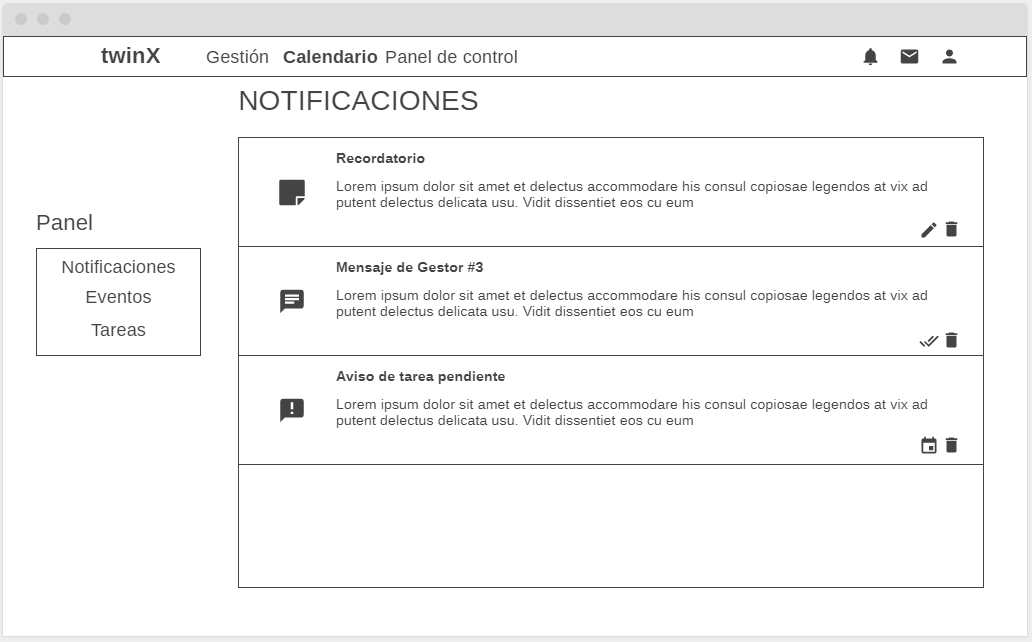
\includegraphics[width=\textwidth]{img/Wireframes/Calendario/notificaciones_lista.png}
	\caption[Wireframe de lista de notificaciones]{Wireframe de lista de notificaciones. Pueden aparecer tres tipos de notificaciones, dependiendo del tipo de mensaje recibido o generado por la propia plataforma (a través de avisos y/o recordatorios)}
	\label{fig:notificaciones_listaWF}
\end{figure}

\begin{figure}
	\centering
	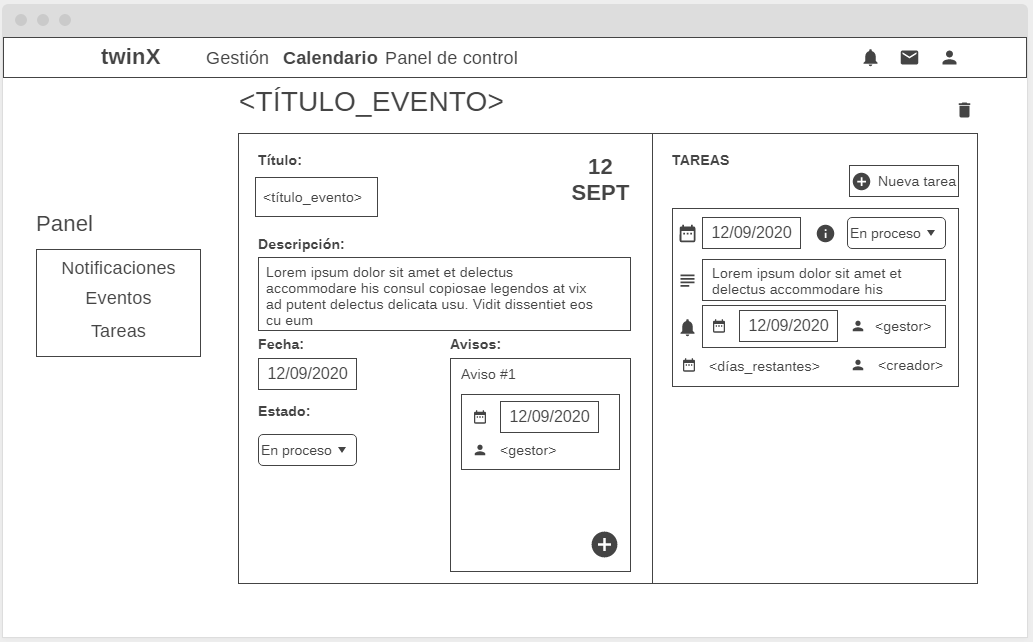
\includegraphics[width=\textwidth]{img/Wireframes/Calendario/nuevo_evento.png}
	\caption[Wireframe de creación de un evento]{Wireframe de creación de un evento. Se distinguen dos vistas: la información del evento en general (izquierda) y la de sus subtareas (derecha)}
	\label{fig:nuevo_eventoWF}
\end{figure}



